Dans ce chapitre, nous décrivons la mise en œuvre des analyses statiques
précédentes. Nous commençons par un tour d'horizon des représentations
intermédiaires possibles, avant de décrire celle retenue : Newspeak. La chaîne
de compilation est explicitée, partant de C pour aller au langage impératif
décrit dans le chapitre~\ref{cha:lang}. Enfin, nous donnons les détails d'un
algorithme d'inférence de types à la Hindley-Milner, reposant sur l'unification
et le partage de références.

\section{Langages intermédiaires}

Le langage C \cite{KandR,AnsiC} a été conçu pour être une sorte d'assembleur
portable, permettant décrire du code indépendamment de l'architecture sur
laquelle il sera compilé. Historiquement, c'est il a permis de créer Unix, et
ainsi de nombreux logiciels bas niveau sont écrits en C. En particulier, il
existe des compilateurs de C vers les différents langages machine pour à peu
près toutes les architectures.

\begin{figure}
  \centering

  \begin{tikzpicture}
  \node[draw] (me) {Langage intermédiaire};
  \node[draw,  above left of=me, xshift=-4cm] (fe1) {Langage source 1};
  \node[draw,  below left of=me, xshift=-4cm] (fe2) {Langage source 2};
  \node[draw, above right of=me, xshift=4cm] (be1) {Langage destination 1};
  \node[draw, below right of=me, xshift=4cm] (be2) {Langage destination 2};

  \draw[->] (fe1) -- (me);
  \draw[->] (fe2) -- (me);

  \draw[->] (me) -- (be1);
  \draw[->] (me) -- (be2);

  \path (me) edge [loop below] node {Optimisations, analyses} (me);

  \coordinate (legbase) at ($ (me) + (0,-2cm) $);

  \draw[bigbrace] (me.south east |- legbase)
               to node [yshift=-5mm] {Middle-end}
                  (me.south west |- legbase);
  \draw[bigbrace] (me.south west |- legbase)
               to node [yshift=-5mm]{Front-end}
                  (fe2.south west |- legbase);
  \draw[bigbrace] (be2.south east |- legbase)
               to node [yshift=-5mm]{Back-end}
                  (me.south east |- legbase);
\end{tikzpicture}


  \caption{Décomposition d'un compilateur : front-ends, middle-end, back-ends}
  \label{fig:middle-end}
\end{figure}

Lors de l'écriture d'un compilateur, on a besoin d'un langage intermédiaire qui
fasse l'intermédiaire entre \emph{front-end} et \emph{back-end}
(figure~\ref{fig:middle-end}). Depuis ce langage on doit pouvoir exprimer des
transformations intermédiaires sur cette représentation (analyses sémantiques,
optimisations, etc), mais aussi compiler ce langage vers un langage machine.

L'idée de prendre C comme langage intermédiaire est très séduisante, mais
malheureusement sa sémantique est trop complexe et trop peu spécifiée. Il est
donc judicieux d'utiliser un langage plus simple à cet effet. Dans de nombreux
projets, des sous-ensembles de C ont été définis pour aller dans ce sens.

\subsubsection{Langages}

Les premiers candidats sont bien entendu les représentations intermédiaires
utilisées dans les compilateurs C. Elles ont l'avantage d'accepter en plus du C
standard, les diverses extensions (GNU, Microsoft, Plan9) utilisées par la
plupart des logiciels. En particulier, le noyau Linux repose fortement sur les
extensions GNU.

\paragraph{GCC} utilise une représentation interne nommée
GIMPLE\cite{gcc-gimple}. Il s'agit d'une structure d'arbre écrite en C, reposant
sur de nombreuses macros afin de cacher les détails d'implémentation pouvant
varier entre deux versions de GCC. Cette représentation étant réputée difficile
à manipuler, le projet MELT\cite{gcc-melt} permet de générer une passe de
compilation à partir d'un dialecte de Lisp.

\paragraph{LLVM}\cite{llvm-pres} est un compilateur développé par la communauté
puis sponsorisé Apple. À la différence de GCC, sa base de code est écrite en
C++. Il utilise une représentation intermédiaire qui peut être manipulée soit
sous forme d'une structure de données C++, soit d'un fichier de code-octet
compact, soit sous forme textuelle.

\paragraph{Objective Caml}\link{ocamlManual} utilise pour sa génération de code
une représentation interne nommée Cmm, disponible dans les sources du
compilateur sous le chemin \texttt{asmcomp/cmm.mli} (il s'agit donc d'une
structure de données OCaml). Ce langage a l'avantage d'être très restreint, mais
malheureusement il n'existe pas directement de traducteur permettant de compiler
C vers Cmm.

\paragraph{C--}\cite{spjcmm} \link{cmm}, dont le nom est inspiré du précédent,
est un projet qui visait à unifier les langages intermédiaires utilisés par les
compilateurs. L'idée est que si un front-end peut émettre du C-- (sous forme de
texte), il est possible d'obtenir du code machine efficace. Le compilateur
Haskell GHC utilise une représentation intermédiaire très similaire à C--.

Comme le problème de construire une représentation intermédiaire adaptée à une
analyse statique n'est pas nouveau, plusieurs projets ont déjà essayé d'y
apporter une solution. Puisque qu'ils sont développés en parallèle des
compilateurs, le support des extensions est en général moins important dans ces
langages.

\paragraph{CIL}\cite{NeculaCil} \link{kerneisCil} est une représentation en
OCaml d'un programme C, développée depuis 2002. Grâce à un mécanisme de
greffons, elle permet de prototyper rapidement des analyses statiques de
programmes.

\paragraph{Newspeak}\cite{newspeak} est un langage intermédiaire développé par
EADS Innovation Works, et qui est spécialisé dans l'analyse de valeurs par
interprétation abstraite. Il sera décrit plus en détails dans la
section~\ref{sec:npk}.

\paragraph{Compcert} est un projet qui vise à produire un compilateur certifié
pour C. C'est à dire que le fait que les transformations conservent la
sémantique est prouvé. Il utilise de nombreux langages intermédiaires, dont CIL.
Pour le front-end, le langage se nomme Clight\cite{cfront}. Les passes de
middle-end, quant à elles, utilisent Cminor\cite{cminorSL}.

%\begin{tabular}{| l || l | l | l | l | l | l |}
\hline
Nom           & Langage hôte    & Description       & But                 & Langage source                   &  Sémantique & Types \\ \hline \hline
C             & Texte           & \cite{AnsiC}      & Compilation         & C                                &  Non        & Oui   \\ \hline
GIMPLE        & C               & \cite{gcc-gimple} & Compilation         & C + extensions, C++, Ada, \ldots &  Non        & Non   \\ \hline
LLVM          & C++             & \cite{llvm-pres}  & Compilation         & C + extensions, C++, Ada, \ldots &             & Oui   \\ \hline
Cminusminus   & Texte           & \cite{spjcmm}     & Compilation         &                                  &             & Oui   \\ \hline
Cmm (Haskell) & Texte / Haskell &                   & Compilation         &                                  &             &       \\ \hline
Cmm (OCaml)   & OCaml           &                   & Compilation         &                                  &             &       \\ \hline
CIL           & OCaml           & \cite{NeculaCil}  & Analyse             &                                  &             &       \\ \hline
Clight        & Coq             & \cite{cfront}     & Compilation/Analyse &                                  &  Oui        & Oui   \\ \hline
Cminor        & Coq             & \cite{cminorSL}   & Compilation/Analyse &                                  &  Oui        & Oui   \\ \hline
Newspeak      & Ocaml           & \cite{newspeak}   & Analyse             &                                  &  Oui        & Oui   \\ \hline
\end{tabular}

% vim: textwidth=0


\section{Newspeak}
\label{sec:npk}

\wip{}

\section{Chaîne de compilation}

\begin{figure}
  \centering
  \begin{tikzpicture}\shorthandoff{!}
\tikzstyle{file}=[draw, shape=rectangle, node distance=2.2cm, minimum
height=1cm, shade, top color=white,
    bottom color=blue!50!black!20, draw=blue!40!black!60, very thick];

\node [file] (c1) {\textcolor{black}{.c}};
\node [file, below of=c1] (c2) {\textcolor{black}{.c}};
\node [node distance=2.2cm, below of=c2] (c3) {};

\node [file, minimum height=0, node distance=5mm, above of=c3,draw] (c3b) {.adb};
\node [file, minimum height=0, node distance=5mm, below of=c3,draw] (c3s) {.ads};

\path (c3b.north west) ++(-3mm,3mm) [draw,dotted] rectangle ($(c3s.south east)+(3mm,-3mm)$);

\node [below of=c3, node distance=2.2cm] (c4){};

\node [file, right of=c1] (cc1) {\textcolor{black}{.c}};
\node [file, right of=c2] (cc2) {\textcolor{black}{.c}};
\node [node distance=2.2cm, right of=c3] (cc3) {};

\node [below of=cc3, node distance=2.2cm](cc4){};

\draw[->] (c1) -- node[above] {{\tiny \ttfamily cpp}} (cc1);
\draw[->] (c2) -- (cc2);

\node [file, right of=cc1] (no1) {\textcolor{black}{.no}};
\node [file, right of=cc2] (no2) {\textcolor{black}{.no}};
\node [file, right of=cc3] (no3) {\textcolor{black}{.no}};

\node [below of=no3, node distance=2.2cm](no4){};

\draw[->] (cc1) -- node[above] {{\tiny \ttfamily c2newspeak -c}} (no1);
\draw[->] (cc2) --  (no2);

\draw[->] ($ (c3b.north east)!0.5!(c3s.south east) + (3mm,0) $) -- node[above] {\tiny \ttfamily ada2newspeak -c} (no3);


\node [file, right of=no2] (npk) {\textcolor{black}{.npk}};

\node [right of=no3, node distance=2.2cm](npk2){};
\node [right of=no4, node distance=2.2cm](npk3){};

\node[draw, ellipse, right of=no2, minimum height=3cm]{};

\draw[->] (no1) -- node {} (npk);
\draw[->] (no2) -- node[above] {{\tiny \ttfamily c2newspeak}} (npk);
\draw[->] (no3) -- node {} (npk);


\node [file, right of=npk, node distance=3cm, yshift=1cm](warn)
    {\textcolor{black}{\parbox{2cm}{\centering Programme \linebreak typé}}};
\node [right of=npk, node distance=3cm, yshift=-1cm](warnn)
    {\textcolor{black}{Erreurs}};

\node [right of=npk3, node distance=3cm](analyser2){};

\node [right of=npk, node distance=3cm] {\small ou};

\draw[->] (npk) -- node[above, yshift=2mm] {{\tiny \ttfamily ptrtype}} (warn);

\draw[->] (npk) -- (warnn);

\draw[->] (c4)   -- node[above, text depth=3pt] {\footnotesize Pr\'etraitement} (cc4);
\draw[->] (cc4)  -- node[above, text depth=3pt] {\footnotesize Compilation} (no4);
\draw[->] (no4)  -- node[above, text depth=3pt] {\footnotesize \'Edition de liens} (npk3);
\draw[->] (npk3) -- node[above, text depth=3pt] {\footnotesize Analyse} (analyser2);
\end{tikzpicture}

  \caption{Compilation depuis Newspeak}
  \label{fig:compil-npk}
\end{figure}

\todo{Mettre à jour la figure}

La compilation vers C est faite en trois étapes (figure~\ref{fig:compil-npk}) :
prétraitement du code source, compilation de C prétraité vers \newspeak{}, puis
compilation de \newspeak{} vers ce langage.

\subsection{Prétraitement}

\ctonewspeak{} travaillant uniquement sur du code prétraité (dans directives de
préprocesseur), la première étape consiste donc à faire passer le code par \cpp:
les macros sont développées, les constantes remplacées par leurs valeurs, les
commentaires supprimés, les fichiers d'en-tête inclus, etc.

\subsection{Compilation (levée des ambigüités)}

Cette passe est réalisée par l'utilitaire \ctonewspeak{}. L'essentiel de la
compilation consiste à mettre à plat les définition de types, et à simplifier le
flot de contrôle. C en effet propose de nombreuses constructions ambigües ou
redondantes.

Au contraire, \newspeak{} propose un nombre réduit de constructions. Rappelons
que le but de ce langage est de faciliter l'analyse statique : des constructions
orthogonales permettent donc d'éviter la duplication de règles sémantique, ou de
code lors de l'implémentation d'un analyseur.

Par exemple, plutôt que de fournir une boucle \emph{while}, une boucle
\emph{do/while} et une boucle for, \newspeak{} fournit une unique boucle
\npkWhile{}. La sortie de boucle est compilée vers un \npkGoto{}, qui est
toujours un saut vers l'avant (similaire à un "break" généralisé).

La sémantique de \newspeak{} et la traduction de C vers \newspeak{} sont
décrites dans \cite{newspeak}. En ce qui concerne l'élimination des sauts vers
l'arrière, on peut se référer à \cite{goto}.

\subsection{Annotations}

\newspeak{} a de nombreux avantages, mais pour une analyse par typage il est
trop bas niveau. Par exemple, dans le code suivant

\begin{Verbatim}[commandchars=\\\{\}]
\PY{k}{struct} \PY{n}{s} \PY{p}{\PYZob{}}
    \PY{k+kt}{int} \PY{n}{a}\PY{p}{;}
    \PY{k+kt}{int} \PY{n}{b}\PY{p}{;}
\PY{p}{\PYZcb{}}\PY{p}{;}

\PY{k+kt}{int} \PY{n+nf}{main}\PY{p}{(}\PY{k+kt}{void}\PY{p}{)}
\PY{p}{\PYZob{}}
    \PY{k}{struct} \PY{n}{s} \PY{n}{x}\PY{p}{;}
    \PY{k+kt}{int} \PY{n}{y}\PY{p}{[}\PY{l+m+mi}{10}\PY{p}{]}\PY{p}{;}
    \PY{n}{x}\PY{p}{.}\PY{n}{b} \PY{o}{=} \PY{l+m+mi}{1}\PY{p}{;}
    \PY{n}{y}\PY{p}{[}\PY{l+m+mi}{1}\PY{p}{]} \PY{o}{=} \PY{l+m+mi}{1}\PY{p}{;}
    \PY{k}{return} \PY{l+m+mi}{0}\PY{p}{;}
\PY{p}{\PYZcb{}}
\end{Verbatim}


\wip{}

\subsection{Implantation de l'algorithme de typage}

Commençons par étudier le cas du lambda-calcul simplement typé
(figure~\ref{fig:stlc}).

\begin{figure}

\gramlr{Termes}{
\begin{align*}
  t \gramisa & x              & \textrm{Variable} \\
    \gramor  & λ x . t        & \textrm{Abstraction} \\
    \gramor  & t              & \textrm{Application} \\
    \gramor  & n              & \textrm{Entier} \\
    \gramor  & f              & \textrm{Flottant} \\
    \gramor  & (t, t)         & \textrm{Couple} \\
    \gramor  & \textrm{fst}~t & \textrm{Projection gauche} \\
    \gramor  & \textrm{snd}~t & \textrm{Projection droite}
\end{align*}
}

\gramlr{Types}{
\begin{align*}
  τ \gramisa &  \tInt          & \textrm{Entier}\\
    \gramor  &  \tFloat        & \textrm{Flottant}\\
    \gramor  & τ \rightarrow τ & \textrm{Fonction} \\
    \gramor  & τ \times τ      & \textrm{Produit}
\end{align*}
}

\gramlr{Contextes}{
\begin{align*}
  Γ \gramisa & ε     & \textrm{Contexte vide}\\
    \gramor  & Γ,x:τ & \textrm{Extension}
\end{align*}
}

\gramlr{Règles}{
\begin{mathpar}
\irule{Int}{ }{Γ⊢n:\tInt}
\and
\irule{Float}{ }{Γ⊢f:\tFloat}
\and
\irule{Var}{x:τ∈Γ}{Γ⊢x:τ}
\and
\irule{App}{Γ⊢f:τ_1 \rightarrow τ_2 \\ Γ ⊢ x : τ_1}{Γ ⊢ f x : τ_2}
\and
\irule{Abs}{Γ,x:τ_1⊢ y : τ_2}{Γ⊢ λx.y:τ_1 \rightarrow τ_2}
\and
\irule{Proj-g}{Γ⊢x:τ_1\times τ_2}{Γ⊢\textrm{fst}~x:τ_1}
\and
\irule{Proj-d}{Γ⊢x:τ_1\times τ_2}{Γ⊢\textrm{snd}~x:τ_2}
\and
\irule{Tup}{Γ⊢x:τ_1 \\ Γ⊢y:τ_2}{Γ⊢(x,y):τ_1 \times τ_2}
\end{mathpar}
}


\caption{Lambda calcul simplement typé avec entiers, flottants et couples}
\label{fig:stlc}

\end{figure}

Prenons l'exemple de la fonction suivante\footnote{ On suppose que \texttt{plus}
est une fonction de l'environnement global qui a pour type $\tInt \rightarrow
\tInt \rightarrow \tInt$.} :

\[
f = λx.λy. \textrm{plus} (\textrm{plus} (\textrm{fst} x) (\textrm{snd} x)) y
\]

On voit que puisque \texttt{fst} et \texttt{snd} sont appliqués à \texttt{x}, ce
doit être un tuple. En outre on additionne ces deux composantes ensemble, donc
elles doivent être de type \tInt (et le résultat aussi). Par le même argument,
\texttt{y} doit aussi être de type \tInt. En conclusion, \texttt{x} est de type
$\tInt \times \tInt$ et \texttt{y} de type $\tInt$, donc f est de type $\tInt
\times \tInt \rightarrow \tInt \rightarrow \tInt$.

Mais comment faire pour implanter cette analyse ? En fait le système de types de
la figure~\ref{fig:stlc} a une propriété particulièrement intéressante : chaque
forme syntaxique (variable, abstraction, etc) est en conclusion exactement d'une
règle de typage. Cela permet de toujours savoir quelle règle il faut appliquer.

Partant du terme de conclusion ($f$), on peut donc en déduire un squelette
d'arbre d'inférence (figure~\ref{fig:inftree-rules})\footnote{Par souci de
clarté, les prémisses des applications de \textsc{(Var)} ne sont pas notées.}

\begin{figure} % {{{ Fig règles
\def\disptypeL#1{}
\def\disptypeR#1{}

\def\gammaXY{\ensuremath{Γ_2}}
\def\gammaX{\ensuremath{Γ_1}}
\def\gammaOneDef{\ensuremath{Γ^0, x\disptypeL{\tInt \times \tInt}, y\disptypeL{\tInt}}}
\def\gammaTwoDef{\ensuremath{Γ^0, x\disptypeL{\tInt \times \tInt}}}
\def\termFst#1{\ensuremath{\textrm{fst}~x}}
\def\termSnd#1{\ensuremath{\textrm{snd}~x}}
\def\fstx{\termFst{x}}
\def\sndx{\termSnd{x}}
\begin{mathpar}
\irule
  {Abs}
  {
    \irule
      {Abs}
      {
        \inferrule*[right=(App)]
          {
            \inferrule*[right=(Var), rightskip=4em]
              { }
              {\gammaXY ⊢ y
              \disptypeR{\tInt}
              }
            \\
            \inferrule*[right=(App),vdots=4em,leftskip=5em,rightskip=5em]
              {
                \inferrule*[right=(Var), leftskip=3em, rightskip=7em]
                  { }
                  {\gammaXY ⊢ \textrm{plus}
                  \disptypeR{\tInt \rightarrow \tInt \rightarrow \tInt}
                  }
                \\
                \inferrule*[right=(App),vdots=3em,leftskip=7em,rightskip=3em]
                  {
                    \inferrule*[right=(App), vdots=4em, rightskip=5em]
                      {
                        \inferrule*[right=(Var), rightskip=5em]
                          { }
                          {\gammaXY ⊢ \textrm{plus}
                          \disptypeR{\tInt \rightarrow \tInt \rightarrow \tInt}
                          }
                        \\
                        \inferrule*[right=(Proj-G), vdots=3em, leftskip=5em]
                          {
                            \irule
                              {Var}
                              { }
                              {\gammaXY ⊢ x
                              \disptypeR{\tInt \times \tInt}
                              }
                          }
                          {\gammaXY ⊢ \fstx
                          \disptypeR{\tInt}
                          }
                      }
                      {\gammaXY ⊢ \textrm{plus} (\fstx)
                      \disptypeR{\tInt \rightarrow \tInt}
                      }
                    \\
                    \inferrule*[right=(Proj-D), leftskip=5em, rightskip=4em]
                      {
                        \irule
                          {Var}
                          { }
                          {\gammaXY ⊢ x
                          \disptypeR{\tInt \times \tInt}
                          }
                      }
                      {\gammaXY ⊢ \sndx
                      \disptypeR{\tInt}
                      }
                  }
                  {\gammaXY ⊢ \textrm{plus} (\fstx) (\sndx)
                  \disptypeR{\tInt}
                  }
              }
              {\gammaXY ⊢ \textrm{plus} (\textrm{plus} (\fstx) (\sndx))
              \disptypeR{\tInt \rightarrow \tInt}
              }
          }
          {\gammaXY ⊢ \textrm{plus} (\textrm{plus} (\fstx) (\sndx)) y
          \disptypeR{\tInt}
          }
      }
      {\gammaX ⊢ λy. \textrm{plus} (\textrm{plus} (\fstx) (\sndx)) y
      \disptypeR{\tInt \rightarrow \tInt}
      }
  }
  {Γ_0 ⊢ λx.λy. \textrm{plus} (\textrm{plus} (\fstx) (\sndx)) y
  \disptypeR{\tInt \times \tInt \rightarrow \tInt \rightarrow \tInt}
  }
\end{mathpar}

\[\gammaX = \gammaTwoDef \qquad \gammaXY = \gammaOneDef\]


\caption{Arbre d'inférence : règles à utiliser}
\label{fig:inftree-rules}
\end{figure} % }}}

\begin{figure} % {{{ Fig full tree
\def\disptypeL#1{:#1}
\def\disptypeR#1{:#1}

\def\gammaXY{\ensuremath{Γ_2}}
\def\gammaX{\ensuremath{Γ_1}}
\def\gammaOneDef{\ensuremath{Γ^0, x\disptypeL{\tInt \times \tInt}, y\disptypeL{\tInt}}}
\def\gammaTwoDef{\ensuremath{Γ^0, x\disptypeL{\tInt \times \tInt}}}
\def\termFst#1{\ensuremath{\textrm{fst}~x}}
\def\termSnd#1{\ensuremath{\textrm{snd}~x}}
\def\fstx{\termFst{x}}
\def\sndx{\termSnd{x}}
\begin{mathpar}
\irule
  {Abs}
  {
    \irule
      {Abs}
      {
        \inferrule*[right=(App)]
          {
            \inferrule*[right=(Var), rightskip=4em]
              { }
              {\gammaXY ⊢ y
              \disptypeR{\tInt}
              }
            \\
            \inferrule*[right=(App),vdots=4em,leftskip=5em,rightskip=5em]
              {
                \inferrule*[right=(Var), leftskip=3em, rightskip=7em]
                  { }
                  {\gammaXY ⊢ \textrm{plus}
                  \disptypeR{\tInt \rightarrow \tInt \rightarrow \tInt}
                  }
                \\
                \inferrule*[right=(App),vdots=3em,leftskip=7em,rightskip=3em]
                  {
                    \inferrule*[right=(App), vdots=4em, rightskip=5em]
                      {
                        \inferrule*[right=(Var), rightskip=5em]
                          { }
                          {\gammaXY ⊢ \textrm{plus}
                          \disptypeR{\tInt \rightarrow \tInt \rightarrow \tInt}
                          }
                        \\
                        \inferrule*[right=(Proj-G), vdots=3em, leftskip=5em]
                          {
                            \irule
                              {Var}
                              { }
                              {\gammaXY ⊢ x
                              \disptypeR{\tInt \times \tInt}
                              }
                          }
                          {\gammaXY ⊢ \fstx
                          \disptypeR{\tInt}
                          }
                      }
                      {\gammaXY ⊢ \textrm{plus} (\fstx)
                      \disptypeR{\tInt \rightarrow \tInt}
                      }
                    \\
                    \inferrule*[right=(Proj-D), leftskip=5em, rightskip=4em]
                      {
                        \irule
                          {Var}
                          { }
                          {\gammaXY ⊢ x
                          \disptypeR{\tInt \times \tInt}
                          }
                      }
                      {\gammaXY ⊢ \sndx
                      \disptypeR{\tInt}
                      }
                  }
                  {\gammaXY ⊢ \textrm{plus} (\fstx) (\sndx)
                  \disptypeR{\tInt}
                  }
              }
              {\gammaXY ⊢ \textrm{plus} (\textrm{plus} (\fstx) (\sndx))
              \disptypeR{\tInt \rightarrow \tInt}
              }
          }
          {\gammaXY ⊢ \textrm{plus} (\textrm{plus} (\fstx) (\sndx)) y
          \disptypeR{\tInt}
          }
      }
      {\gammaX ⊢ λy. \textrm{plus} (\textrm{plus} (\fstx) (\sndx)) y
      \disptypeR{\tInt \rightarrow \tInt}
      }
  }
  {Γ_0 ⊢ λx.λy. \textrm{plus} (\textrm{plus} (\fstx) (\sndx)) y
  \disptypeR{\tInt \times \tInt \rightarrow \tInt \rightarrow \tInt}
  }
\end{mathpar}

\[\gammaX = \gammaTwoDef \qquad \gammaXY = \gammaOneDef\]


\caption{Arbre d'inférence complet}
\label{fig:inftree-full}
\end{figure} % }}}

Une fois à cette étape, on peut donner un nom à chaque type inconnu : $τ_1, τ_2,
\ldots$. L'utilisation qui en est faite permet de générer un ensemble de
contraintes d'unification. Par exemple, pour chaque application de la règle
\textsc{(App)} :

\[
\irule{App}{Γ⊢\ldots:τ_3 \\ Γ ⊢ \ldots : τ_1}{Γ ⊢ \ldots : τ_2}
\]

on doit déduire que $τ_3 = τ_1 \rightarrow τ_2$.

\clearpage

Ce signe $=$ est à prendre comme une contrainte d'égalité : partant d'un
ensemble de contraintes de la forme "type avec inconnue = type avec inconnue",
on veut obtenir une substitution "inconnue -> type concret".

Pour résoudre ces contraintes, on commence par les simplifier : si $τ_a
\rightarrow τ_b = τ_c \rightarrow τ_d$, alors $τ_a = τ_c$ et $τ_b = τ_d$. De
même si $τ_a \times τ_b = τ_c \times τ_d$. Au contraire, si $τ_a \rightarrow τ_b
= τ_c \times τ_d$, il est impossible d'unifier les types et il faut abandonner
l'inférence de types. D'autre cas sont impossibles, par exemple $\tInt = τ_1
\rightarrow τ_2$ ou $\tInt = \tFloat$.

Une fois ces simplifications réalisées, les contraintes restantes sont d'une des
formes suivantes :

\begin{itemize}
\item
  $τ_i = τ_i$. Il n'y a rien à faire, cette contrainte peut être supprimée.
\item
  $τ_i = τ_j$ avec $i \ne j$ : toutes les occurrences de $τ_j$ dans les autres
  contraintes peuvent être remplacées par $τ_i$.
\item
  $τ_i = x$ (ou $x = τ_i$) où $x$ est un type concret : idem.
\end{itemize}

\todo{C'est faux}

Une fois toutes les substitutions effectuées, on obtient un arbre de typage
correct (figure~\ref{fig:inftree-full}, donc un programme totalement inféré.

\clearpage

\begin{figure} % fig:unifpartage {{{

  \subfloat[][]{
  \label{fig:unifpartage:a}
  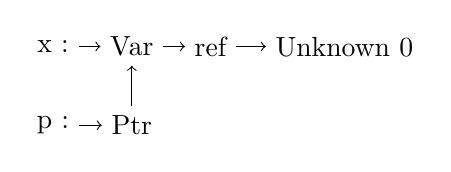
\begin{tikzpicture}
  \node               (var) {Var};
  \node[right of=var] (ref) {ref};
  \node[right of=ref, node distance=1.7cm] (u0) {Unknown 0};
  \node[below of=var] (ptr) {Ptr};
  \node[left of=var]  (x) {x :};
  \node[left of=ptr] (p) {p :};
  \draw[->] (x) -- (var);
  \draw[->] (p) -- (ptr);
  \draw[->] (ptr) -- (var);
  \draw[->] (var) -- (ref);
  \draw[->] (ref) -- (u0);
  \end{tikzpicture}
  }
  \subfloat[][]{
  \label{fig:unifpartage:b}
  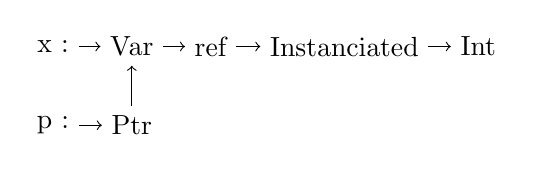
\begin{tikzpicture}
  \node               (var) {Var};
  \node[right of=var] (ref) {ref};
  \node[right of=ref, node distance=1.7cm] (u0) {Instanciated};
  \node[right of=u0, node distance=1.7cm] (ii) {Int};
  \node[below of=var] (ptr) {Ptr};
  \node[left of=var]  (x) {x :};
  \node[left of=ptr] (p) {p :};
  \draw[->] (x) -- (var);
  \draw[->] (p) -- (ptr);
  \draw[->] (ptr) -- (var);
  \draw[->] (var) -- (ref);
  \draw[->] (ref) -- (u0);
  \draw[->] (u0) -- (ii);
  \end{tikzpicture}
  }
  \subfloat[][]{
  \label{fig:unifpartage:c}
  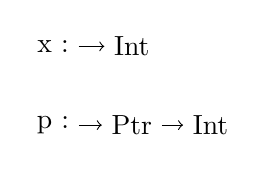
\begin{tikzpicture}
  \node               (var) {Int};
  \node[below of=var] (ptr) {Ptr};
  \node[left of=var]  (x) {x :};
  \node[left of=ptr] (p) {p :};
  \node[right of=ptr] (pi) {Int};
  \draw[->] (x) -- (var);
  \draw[->] (p) -- (ptr);
  \draw[->] (ptr) -- (pi);
  \end{tikzpicture}
  }

  \caption{Unification par partage}
  \label{fig:unifpartage}

\end{figure} % }}}

Plutôt que de modifier toutes les occurrences d'un type $τ_i$, on va affecter à
$τ_i$ la valeur du nouveau type.

L'implémentation de cet algorithme utilise le partage et les références
(figure~\ref{fig:unifpartage}).

D'abord \ref{fig:unifpartage:a}, ensuite \ref{fig:unifpartage:b}, et enfin
\ref{fig:unifpartage:c}.

\begin{figure} % fig:exunif:c {{{

  \insertcode{ex-unif-c.c}

  \caption{Compilation d'un programme C - avant}
  \label{fig:exunif:c}
\end{figure} % }}}

Prenons l'exemple de la figure~\ref{fig:exunif:c} et typons-le "à la main". On
commence par oublier toutes les étiquettes de type présentes dans le programme.
Celui-ci devient alors :

\begin{Verbatim}
var x, p;
p = &x;
x = 0;
\end{Verbatim}

La premiere ligne introduit deux variables. On peut noter leurs types respectifs
(inconnus pour le moment) $t_1$ et $t_2$. La première affectation \texttt{p =
\&x} implique que les deux côtés du signe "=" ont le même type. À gauche, le
type est $t_2$, et à droite $Ptr(t_1)$. On applique le même raisonnement à la
seconde affectation : à gauche, le type est $t_1$ et à droite Int. On en déduit
que le type de x est Int et celui de p est Ptr(Int).


\insertcode{lambda-types.ml}

Pour implanter cet algorithme, on représente les types de données du programmes
à typer par une valeur de type \texttt{ml\_type}. En plus des constantes de
types comme int ou float, et des constructeurs de type comme pair et fun, le
constructeur Var permet d'exprimer les variables de types (inconnues ou non).

Celles-ci sont numérotées par un int, on suppose avoir à disposition deux
fonctions manipulant un compteur global d'inconnues.

\begin{Verbatim}
module Counter : sig
  val reset_unknowns : unit -> unit
  val new_unknown : unit -> int
end
\end{Verbatim}

De plus, on a un module gérant les environnements de typage. Il pourra être
implanté avec des listes d'association ou des tables de hachage, par exemple. Sa
signature est :

\begin{Verbatim}
module Env : sig
  type t

  (* Construction *)
  val empty : t
  val extend : ml_ident -> ml_type -> t -> t

  (* Interrogation *)
  val get : ml_ident -> t -> ml_type option
end
\end{Verbatim}

Reprenons l'exemple précédent. Partant d'un environnement vide (Env.empty), on
commence par l'étendre de deux variables. Comme on n'a aucune information, il
fait allouer des nouveaux noms d'inconnues (qui correspondent à $t_1$ et $t_2$):

\begin{Verbatim}
let t1 = Var_type (Unknown (new_unknown ())) in
let t2 = Var_type (Unknown (new_unknown ())) in
let env =
  Env.extend "p" t2
    (Env.extend "x" t1
      Env.empty
    ) in
\end{Verbatim}

La première instruction indique que les deux côtés de l'affectation doivent
avoir le même type.

\begin{Verbatim}
let lhs1 = Lv_var "p"
and rhs1 = AddrOf (Exp_var "x") in
let t_lhs1 = typeof lhs1 env
and t_rhs1 = typeof rhs1 env in
unify t_lhs1 t_rhs1;
\end{Verbatim}

Ici il se passe plusieurs choses intéréssantes. D'une part nous faisont appel à
une fonction externe typeof qui retourne le type d'une expression sous un
environnement (dans une implantation complète il s'agirait d'un appel récursif).
Dans ce cas, \texttt{typeof lhs1 env} est identique à \texttt{Env.get lhs1 env}
et \texttt{typeof rhs1 env} à \texttt{Ptr\_type t1}. L'autre aspect intéressant
est la dernière ligne : la fonction \texttt{unify} va modifier en place les
représentations des types afin de les rendre égales. L'implantation de
\texttt{unify} sera décrite plus tard. Dans ce cas précis, elle va faire pointer
la référence dans t2 vers t1.

\begin{Verbatim}
t1 : Var_type -> ref -> Unknown 0
        ^
        |
        +-------------------------+
                                  |
t2 : Var_type -> Instanciated -> Ptr
\end{Verbatim}

Enfin, la seconde affectation se déroule à peu près de la même manière.

\begin{Verbatim}
let lhs2 = Lv_deref (Lv_var "p")
and rhs2 = Exp_int 0 in
let t_lhs2 = typeof lhs2 env
and t_rhs2 = typeof rhs2 env in
unify t_lhs2 t_rhs2;
\end{Verbatim}

Ici \texttt{typeof lhs2 env} est identique à \texttt{Ptr\_type (Env.get "p"
env)} et \texttt{typeof lhs2 env} à \texttt{Const\_type Int\_type}. Et dans cas,
l'unification doit se faire entre t1 et \texttt{Const\_type Int\_type} : cela
mute la référence derrière t1.

\begin{Verbatim}
t1 : Var_type -> ref -> Instanciated -> Const_type -> Int_type
        ^
        |
        +-------------------------+
                                  |
t2 : Var_type -> Instanciated -> Ptr
\end{Verbatim}

L'essence de l'algorithme d'inférence se situe donc dans 2 fonctions. D'une
part, \texttt{unify} qui réalise l'unification des types grâce à au partage des
références. D'autre part, la \texttt{typeof} qui encode les règles de typage
elles-mêmes et les applique à l'aide de \texttt{unify}.

\subsection{Algorithme d'unification}

Voici une implantation de la fonction \texttt{unify}.

Celle-ci prend en entrée deux types $t_1$ et $t_2$. À l'issue de l'exécution de
\texttt{unify}, ces deux types doivent pouvoir être considérés comme égaux. Si
ce n'est pas possible, une erreur sera levée.

La première étape est de réduire ces deux types, c'est à dire à transformer les
constructions \texttt{Var (ref (Instanciated t))} en \texttt{t}.

Ensuite, cela dépend des formes qu'ont les types réduits :

\begin{itemize}

\item si les deux types sont inconnus (de la forme \texttt{Var (ref
(Instanciated t))}), on fait pointer l'une des deux références vers le premier
type. Notons que cela créé un type de la forme \texttt{Var (ref (Instanciated
(Var (ref (Unknown n)))))} qui sera réduit lors d'une prochaine étape
d'unification.

\item si un type est inconnu et pas l'autre, il faut de la même manière affecter la
référence. Mais en faisant ça inconditionnellement, cela peut poser problème :
par exemple en tentant d'unifier \texttt{a} avec \texttt{Ptr(a)} on pourrait
créer un cycle dans le graphe :

\begin{Verbatim}
Ptr -> Var -> ref -> Instanciated
 ^                         |
 +-------------------------+
\end{Verbatim}

Pour éviter cette situation, il suffit de s'assurer que le type inconnu n'est
pas présent dans le type à affecter.

\item si les deux types sont des types de base (comme \tInt ou \tFloat), on ne
fait rien s'ils sont égaux ; l'algorithme échoue sinon.

\item si les deux types sont des constructeurs de type, il faut que les
constructeurs soient égaux. On unifie en outre leurs arguments deux à deux.

\item TODO sous typage pour les structures

\end{itemize}


TODO :

\begin{itemize}
\item implem du polymorphisme
\item implem du sous-typage
\item généralisation depuis le toy language
\end{itemize}

\clearpage

\begin{figure} % fig:exunif:tpk {{{

  \insertcode{ex-unif-tpk.ml}

  \caption{Compilation d'un programme C - après}
  \label{fig:exunif:tpk}
\end{figure} % }}}

Le programme C (figure~\ref{fig:exunif:c}) est compilé ainsi en Tyspeak
(figure~\ref{fig:exunif:tpk}).

% vim: spelllang=fr
